% Project proposal for the senior design class. Build with:  tectonic project-proposal.tex
% Numbers here come from accelerator/docs (synth_log, memory_map), shopping-list.tex
% and .claude/jonahs-docs. Update them together.

\documentclass[10pt]{article}

\usepackage[margin=0.9in, headheight=14pt]{geometry}
\usepackage[T1]{fontenc}
\usepackage{lmodern}
\usepackage{microtype}
\usepackage{booktabs}
\usepackage{tabularx}
\usepackage{array}
\usepackage{float}
\usepackage{xcolor}
\usepackage{enumitem}
\usepackage{titlesec}
\usepackage{fancyhdr}
\usepackage{caption}
\usepackage{tikz}
\usetikzlibrary{positioning, fit, arrows.meta, shapes.geometric}
\usepackage[colorlinks=true, urlcolor=navy, linkcolor=navy, citecolor=navy]{hyperref}

\definecolor{navy}{HTML}{2B3A67}
\definecolor{bar}{HTML}{8A8FA8}
\definecolor{done}{HTML}{DDE9E1}

\pagestyle{fancy}
\fancyhf{}
\fancyhead[L]{\small\color{gray}Team Manatee}
\fancyhead[R]{\small\color{gray}Autonomous Robotic Chess with a Custom FPGA Inference Accelerator}
\fancyfoot[C]{\small\thepage}
\renewcommand{\headrulewidth}{0.4pt}

\titleformat{\section}{\large\bfseries\color{navy}}{\thesection}{0.6em}{}[{\color{navy!40}\titlerule}]
\titleformat{\subsection}{\normalsize\bfseries\color{navy}}{\thesubsection}{0.6em}{}
\titlespacing*{\section}{0pt}{1.0em}{0.5em}
\titlespacing*{\subsection}{0pt}{0.8em}{0.3em}

\setlength{\parindent}{0pt}
\setlength{\parskip}{0.45em}
\setlist{nosep, leftmargin=1.4em, topsep=0.2em}
\captionsetup{font=small, labelfont=bf, skip=4pt}
\renewcommand{\arraystretch}{1.12}
\newcolumntype{L}{>{\raggedright\arraybackslash}X}
\newcolumntype{P}[1]{>{\raggedright\arraybackslash}p{#1}}
\setlength{\textfloatsep}{8pt}
\setlength{\intextsep}{8pt}

\newcommand{\lead}[1]{\textbf{#1}}

\begin{document}

\begin{center}
{\small\textsc{Tufts University}}\\[0.3em]
\rule{\textwidth}{0.4pt}\\[0.7em]
{\LARGE\bfseries\color{navy} Autonomous Robotic Chess with a\\[0.1em] Custom FPGA Inference Accelerator}\\[0.4em]
{\large Project Proposal}\\[0.3em]
\rule{\textwidth}{0.4pt}
\end{center}

\begin{tabular}{@{}l l}
\textbf{Team:} & Team Manatee \\
\textbf{Team color:} & \textbf{Manatee} \\
\end{tabular}

\begin{tabularx}{\textwidth}{@{}l l L@{}}
\toprule
\textbf{Team member} & \textbf{Tufts email} & \textbf{Team} \\
\midrule
Paul Wang & Paul.Wang@tufts.edu & Robotics, board runtime \\
Jonah Pflaster & Jonah.Pflaster@tufts.edu & Robotics, game software \\
Michael Chou & Michael.Chou664040@tufts.edu & FPGA accelerator \\
Hoang Mai & Hoang.Mai@tufts.edu & FPGA accelerator \\
Matthew Sheng & Matthew.Sheng@tufts.edu & Chess model \\
\midrule
\multicolumn{3}{@{}l}{\textbf{Sponsors:} Dr.\ Bonnie Schnitta (SoundSense) and Dr.\ Samuel Sheng (Google)} \\
\bottomrule
\end{tabularx}

\section{Project Description}

\subsection{Overview}

Our project asks \emph{how good a robot's decisions can be on cheap hardware}. Chess makes
decision quality easy to judge, so we are building a chessboard that plays a full game against a
person. The player moves a piece by hand and presses a button. The board then reads every square,
picks a reply with one pass of a transformer model, and moves its own piece with a Cartesian gantry
and a servo claw. There is no screen or keyboard, because we want it to feel like a normal game of
chess.

Most of the engineering is in the decision step. Everything runs on one AMD Kria KR260~\cite{kr260},
which pairs a quad-core Arm Cortex-A53 (the processing system, PS) with FPGA fabric (the
programmable logic, PL). We are designing our own inference accelerator in the PL for a Maia-style
chess model~\cite{maia, chessformer}, which predicts the move a human of a chosen rating would play.
It uses 8-bit integer weights and 16-bit integer activations. We then run the same network on AMD's
Deep Learning Processor Unit (DPU)~\cite{dpu} and on the CPU alone. All three run on the same board,
so we can compare latency and energy per move and see which operations run in fabric and which fall
back to the CPU. That tells us which operations are worth building custom hardware for.

\begin{table}[H]
\centering\small
\caption{Terms used in this document.}
\begin{tabularx}{\textwidth}{@{}P{2.7cm} L@{}}
\toprule
FPGA / PL / PS & Field-programmable gate array. The KR260's reconfigurable logic (PL) sits beside its Arm processor (PS) on one chip. \\
INT8 / INT16 & 8-bit and 16-bit integer arithmetic, used instead of floating point to make inference small and fast in hardware. \\
DPU & AMD's neural-network accelerator IP for Zynq UltraScale+ devices. It is our baseline. \\
Maia & A family of chess models trained to play like a human at a chosen Elo rating. \\
MAC & Multiply-accumulate, the basic operation of a matrix multiply. One DSP slice on the FPGA does one MAC per clock. \\
G-code & The command language used by 3D printers. We use it to drive the gantry. \\
Golden vectors & Test inputs with known-correct outputs from a bit-accurate software model, used to verify hardware. \\
\bottomrule
\end{tabularx}
\end{table}

\subsection{Updated Description and Requirements}

The scope and the implementation of each subsystem have changed a lot since the initial pitch. Each
change below came from sponsor or mentor feedback.

\begin{itemize}
\item \lead{Scope.} We reframed the project from ``a chess robot'' to an open-source, low-cost
  robotic chessboard that demonstrates an FPGA-accelerated Maia engine.
\item \lead{Platform.} We compared the KR260 with the KD240, a PolarFire SoC, and a microcontroller.
  A microcontroller has no programmable logic, so there would be nothing to accelerate.
\item \lead{Sensing.} We dropped the camera pipeline to keep our time on the accelerator, and
  dropped RFID because of cost. Dr.\ Sheng suggested resistor-coded pieces, which are cheaper and
  simpler than either.
\item \lead{Mechanism.} We compared a gantry, a SCARA arm, CoreXY, and a delta robot. We chose an
  overhead Cartesian gantry because each axis has its own drive, which makes it the simplest to
  build and debug.
\item \lead{Requirements.} We relaxed the turn-time budget from 10~s to 30~s after working out the
  gantry travel times. The board scan must finish within 500~ms, and we are designing for under
  10~ms.
\end{itemize}

Table~\ref{tab:req} lists the requirements that most shape the design. The IDs match the Design
Requirements Document.

\begin{table}[H]
\centering\small
\caption{Key requirements (full list in the Design Requirements Document).}\label{tab:req}
\begin{tabularx}{\textwidth}{@{}P{2.2cm} L P{2.3cm}@{}}
\toprule
\textbf{ID} & \textbf{Requirement} & \textbf{Verified by} \\
\midrule
FR-SEN-1/3 & Report piece type and color (or empty) for all 64 squares; zero misreads over 1,000 scans & Test \\
FR-GAM-2 & Legal-move list matches python-chess on 100\% of at least 10,000 positions & Test \\
FR-ENG-1/2 & Model input matches the reference Maia encoder bit for bit; zero invalid moves selected & Test \\
FR-ACC-3/4 & Accelerator matches the bit-accurate model on every layer; all layers run in PL; timing met & Test, Inspection \\
FR-BEN-1/3/4 & One command benchmarks the custom, DPU, and CPU backends: latency, throughput, energy & Demo, Analysis \\
NFR-1 & Robot turn completes within 30 s of the button press & Test \\
NFR-2 & Engine returns a move within 500 ms (p99) & Test \\
NFR-3 & Every placement within 5 mm of square center over 100 placements & Test \\
NFR-4 & 50 consecutive moves without intervention in 3 of 3 trial runs & Test \\
\bottomrule
\end{tabularx}
\end{table}

\subsection{Assumptions and Dependencies}

\lead{Assumptions.}
\begin{itemize}
\item A small student model distilled from Maia-3 keeps acceptable move-match accuracy with INT8
  weights and INT16 activations. The current candidate has 8 transformer blocks of width 128 and
  about 1.6M weights. Our weight memory for it synthesizes to 49 of the KR260's 64 UltraRAM blocks.
\item If the final model is larger, we can move part of the weights to block RAM or stream them
  from DDR4. The comparison stays valid either way.
\item The player always plays White from the rank-1 side and moves pieces by hand. The robot never
  moves during the player's turn.
\item A resistor in each piece base can be read reliably through a copper-tape contact, despite
  contact resistance.
\end{itemize}

\lead{Dependencies.}
\begin{itemize}
\item \lead{Network specification.} The accelerator's final sizes are blocked until the layer
  shapes, quantization scales, weight layout, and golden vectors are fixed. Until then every size
  in the RTL is a parameter.
\item \lead{External IP and tools.} AMD DPU IP for the baseline, AMD Vivado 2023.2 for synthesis
  and timing, and the public Maia-3 code and weights~\cite{maia3}.
\item \lead{Open-source software.} python-chess as the rules reference, and Marlin G-code
  firmware~\cite{marlin} on the motion controller.
\item \lead{Hardware supply and lab access.} KR260 kit, stepper motors and drivers, rails, a 24~V
  supply, and 3D-printer time.
\item \lead{Sponsor availability} for reviews of the accelerator architecture, the
  energy-measurement method, and the project plan.
\end{itemize}

\subsection{Sponsors}

\lead{Dr.\ Bonnie Schnitta, SoundSense, LLC.} Dr.\ Schnitta is the founder and CEO of SoundSense,
an acoustic engineering firm. She is our mentor and technical reviewer. At each check-in she
reviews progress, questions our methods, and confirms task owners and definitions of done.

\lead{Dr.\ Samuel Sheng, Google.} Dr.\ Sheng is Director of Sensing Technologies at Google and
works in systems design and digital signal processing. He reviews the accelerator architecture and
our energy-measurement method, and advises on sensing. The resistor-coded pieces were his idea, as
was the point that mixed precision is a reason not to rely on the DPU alone.

\subsection{Work to Date}

\lead{Accelerator.} The MAC cell, the $64\times8$ MAC array, the matrix-multiply engine around it,
the activation memory, and the weight memory are written in SystemVerilog. Each passes a
self-checking testbench and meets timing at 100~MHz in out-of-context synthesis. The array uses 512
of the KR260's 1,248 DSP slices. The engine handles weight multiplies and the query-key product of
attention; the attention-value and attention-bias modes are not built yet. The exponential lookup
table for softmax is written and tested, and a DMA loopback test for first board bring-up is
written. The DPU and CPU baselines are in progress.

\lead{Robotics.} The pieces, the claw, and a $2\times2$ test tile are modeled in parametric CAD and
3D printed, and the tile reads the resistor-coded pieces. The gantry is not built yet. The game
software has not been started.

\section{Project Management}

\subsection{Organization and Task Ownership}

Early in the term we spent design time on a camera pipeline, CoreXY, and an NNUE engine, all of
which we dropped. To avoid repeating that, every workstream now has named owners
(Table~\ref{tab:own}), each task has a definition of done, and we review both at sponsor check-ins.
The accelerator and the robot can each be built and tested without the other, because the game
software can run on a CPU backend and in simulation.

\begin{table}[H]
\centering\small
\caption{Workstreams and ownership. The first name leads.}\label{tab:own}
\begin{tabularx}{\textwidth}{@{}P{2.3cm} L P{2.9cm}@{}}
\toprule
\textbf{Workstream} & \textbf{Tasks} & \textbf{Owners} \\
\midrule
Accelerator & Compute core and memories; softmax, normalization, activation, and requantization units; stream adapters and weight loader; block design; PS runtime and board bring-up; DPU and CPU baselines; bit-exact integer reference & Michael, Hoang, Paul \\
Model & Distill and quantize the student model; freeze the architecture and scales; produce golden vectors & Matthew \\
Game software & Game controller state machine, rules engine, board reader, move selector, motion planner; backend API; PGN replay simulation mode; benchmark harness & Jonah, Paul \\
Sensing board & Printed pieces; resistor values and contact design; $2\times2$ test tile; 64-square board with 4 muxes and an ADC; scan firmware & Paul, Jonah \\
Motion and power & Gantry frame, homing, calibration; claw; G-code move generation; 24 V rail, fuse, hardware e-stop & Jonah \\
Project management & Schedule, sponsor check-ins, documentation, budget and BOM, open-source release & Matthew, Jonah \\
\bottomrule
\end{tabularx}
\end{table}

\subsection{Milestones and Schedule}

Table~\ref{tab:ms} lists the major milestones and Figure~\ref{fig:gantt} shows the schedule by month.
Dates after Dec.~4 are our current plan and will be refined once the spring calendar is
set.

\begin{table}[H]
\centering\small
\caption{Major project milestones.}\label{tab:ms}
\begin{tabularx}{\textwidth}{@{}P{2.5cm} L P{1.7cm}@{}}
\toprule
\textbf{Date} & \textbf{Milestone} & \textbf{Status} \\
\midrule
Oct. 26, 2026 & Design Requirements Document (use cases, requirements, user stories) & Complete \\
Nov. 8, 2026 & Initial Technical Design Document (interfaces, architecture, components) & Complete \\
Nov. 20, 2026 & End of Sprint 2: MAC array, matrix-multiply engine, and memories pass simulation; pieces, claw, and test tile printed; tile reads pieces & Complete \\
Dec. 4, 2026 & Design Review and proof-of-concept demo; DPU and CPU baselines measured; model architecture decision & In progress \\
Jan. 2027 & Network spec and golden vectors frozen; special-function units pass simulation; 64-square board built; gantry built and homed & Planned \\
Feb. 2027 & Accelerator runs on KR260 hardware; full game playable on the CPU backend & Planned \\
Mar. 2027 & Custom accelerator bit-exact end to end; DPU and CPU baselines benchmarked & Planned \\
Early Apr. 2027 & \textbf{MVP integration freeze}; 3-of-3 reliability trials & Planned \\
Apr. 2027 & MVP demonstration and benchmark report & Planned \\
\bottomrule
\end{tabularx}
\end{table}

\begin{figure}[H]
\centering
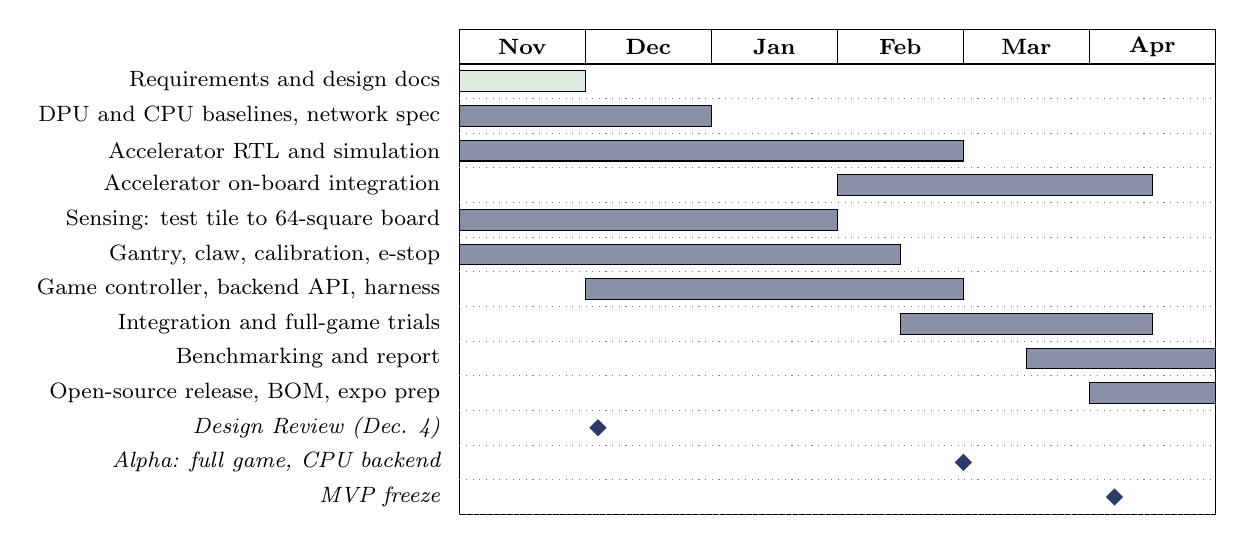
\begin{tikzpicture}[x=0.8cm, y=0.44cm, font=\footnotesize]
  % month headers
  \foreach \m [count=\i from 0] in {Nov, Dec, Jan, Feb, Mar, Apr} {
    \draw (2*\i, 0) rectangle (2*\i+2, 1);
    \node[font=\footnotesize\bfseries] at (2*\i+1, 0.5) {\m};
  }
  \draw (0, 0) rectangle (12, -13);
  % rows: label / start / end / fill
  \foreach \lab/\s/\e/\c [count=\r from 1] in {
    Requirements and design docs/0/2/done,
    {DPU and CPU baselines, network spec}/0/4/bar,
    Accelerator RTL and simulation/0/8/bar,
    Accelerator on-board integration/6/11/bar,
    Sensing: test tile to 64-square board/0/6/bar,
    {Gantry, claw, calibration, e-stop}/0/7/bar,
    {Game controller, backend API, harness}/2/8/bar,
    Integration and full-game trials/7/11/bar,
    Benchmarking and report/9/12/bar,
    {Open-source release, BOM, expo prep}/10/12/bar} {
    \node[anchor=east] at (-0.15, -\r+0.5) {\lab};
    \draw[dotted, gray] (0, -\r) -- (12, -\r);
    \draw[fill=\c] (\s, -\r+0.2) rectangle (\e, -\r+0.8);
  }
  % milestones
  \foreach \lab/\x [count=\r from 11] in {
    Design Review (Dec. 4)/2.2, {Alpha: full game, CPU backend}/8, MVP freeze/10.4} {
    \node[anchor=east, font=\footnotesize\itshape] at (-0.15, -\r+0.5) {\lab};
    \draw[dotted, gray] (0, -\r) -- (12, -\r);
    \node[diamond, fill=navy, inner sep=1.6pt] at (\x, -\r+0.5) {};
  }
\end{tikzpicture}
\caption{Project schedule, Nov.\ 2026 to Apr.\ 2027. Each column is a month. The light bar is
complete and diamonds are milestones.}\label{fig:gantt}
\end{figure}

\subsection{Deliverables to the Sponsors}

\begin{enumerate}[label=D\arabic*., leftmargin=2.2em]
\item A working robotic chessboard that plays a complete game against a human, with the custom
  accelerator choosing each move.
\item The custom accelerator (RTL, bitstream, weights, and bit-accurate software model) with golden
  test vectors.
\item A benchmark report comparing the custom accelerator, the AMD DPU, and the CPU on latency,
  throughput, energy per inference, and fabric utilization. It lists the operations that fall back
  to the CPU and includes any bad or incomplete results.
\item If we complete the model-size sweep, a curve of move-match accuracy against model size.
\item A priced bill of materials with part numbers so others can reproduce the board.
\item Sponsor-facing documents: design requirements, design documents, test results, and a final
  report.
\end{enumerate}

\subsection{Budget}

The KR260 Robotics Starter Kit (\$349) is the one fixed cost. We originally hoped to keep the robot
hardware beyond the KR260 under \$100. The motors, supply, and frame alone exceed that, so we
replaced the cap with NFR-8, which requires us to publish a full priced bill of materials.
Table~\ref{tab:budget} gives planning estimates by group; we will replace them with vendor prices
by the January check-in. A used 3D printer would supply the motors, controller, belts, lead screw,
supply, and limit switches, so we are asking the campus makerspaces for one before buying those
lines.

\begin{table}[H]
\centering\small
\caption{Preliminary budget (planning estimates, USD).}\label{tab:budget}
\begin{tabularx}{\textwidth}{@{}L r@{}}
\toprule
\textbf{Item} & \textbf{Estimate} \\
\midrule
AMD Kria KR260 Robotics Starter Kit (list price) & 349 \\
Motion electronics: 4 NEMA 17 steppers, controller board with 4 drivers, 24 V 150 W supply, fuse, latching e-stop & 120--160 \\
Motion mechanics: belts, pulleys, idlers, lead screw, Z-axis rods and bearings, 3 limit switches & 60--90 \\
Frame: aluminum V-slot extrusion, wheels, brackets, fasteners, plywood base & 80--120 \\
Sensing and pieces: resistors (E24, 1\%), 4 analog mux boards, SPI ADC, copper tape, wire, washers, claw servo, turn button & 50--90 \\
Contingency and spares (about 10\%) & 65--80 \\
\midrule
\textbf{Approximate total} & \textbf{724--889} \\
\bottomrule
\end{tabularx}
\end{table}

\section{Design Choices and Considerations}

\subsection{Background Research: What Already Exists}

\lead{Commercial robotic chessboards.} Consumer boards such as the Square Off line~\cite{squareoff}
move pieces with an XY mechanism and magnets under the board, sense them with embedded electronics,
and play with a conventional engine. Electronic boards from DGT~\cite{dgt} and
Chessnut~\cite{chessnut} detect pieces but do not move them.

\lead{Chess engines and human-like play.} Stockfish~\cite{stockfish} and its NNUE evaluation rely
on deep tree search. AlphaZero~\cite{alphazero} showed strong play from a learned network plus
search, and Deep Blue~\cite{deepblue} is the classic example of custom chess hardware.
Maia~\cite{maia} is different. It is trained to predict the move a human of a given rating would
play, which takes one forward pass and no search. Maia-3 is built on the Chessformer transformer
architecture~\cite{chessformer}. Its attention layers are what make an accelerator for it hard:
softmax, normalization, and a geometric attention bias (GAB) are not natively supported by the DPU.

\lead{Neural-network inference on FPGAs.} Vendor overlays such as the AMD DPU~\cite{dpu} provide a
general INT8 accelerator that streams weights from DDR. They handle convolutional networks well but
run unsupported operations on the CPU. Open frameworks such as FINN~\cite{finn} and
hls4ml~\cite{hls4ml} generate dataflow accelerators for small, latency-critical networks, and
integer-only quantization~\cite{jacob} is the standard route to INT8 inference. Moving data
dominates energy cost in digital systems~\cite{horowitz}, which is why we keep all weights and
activations on chip. We found no open, documented comparison of a custom accelerator against the
DPU for a small attention-based network on a low-cost platform, which is the gap this project tries
to fill.

Complete chess robots exist only as closed commercial products, and published accelerator
comparisons cover other workloads. We are building an open, reproducible board and measuring
custom, vendor, and CPU inference on the same chip.

\subsection{System Diagram}

Figure~\ref{fig:sys} shows the system. The sensing chain (left) converts piece resistances into ADC
codes. The KR260 (center) turns the codes into a board state, chooses a reply, and plans a path.
The motion chain (right) converts G-code into gantry and claw movement. The computer and the motors
have separate supplies, and the emergency stop cuts only motor power, so the game state survives.

\begin{figure}[H]
\centering
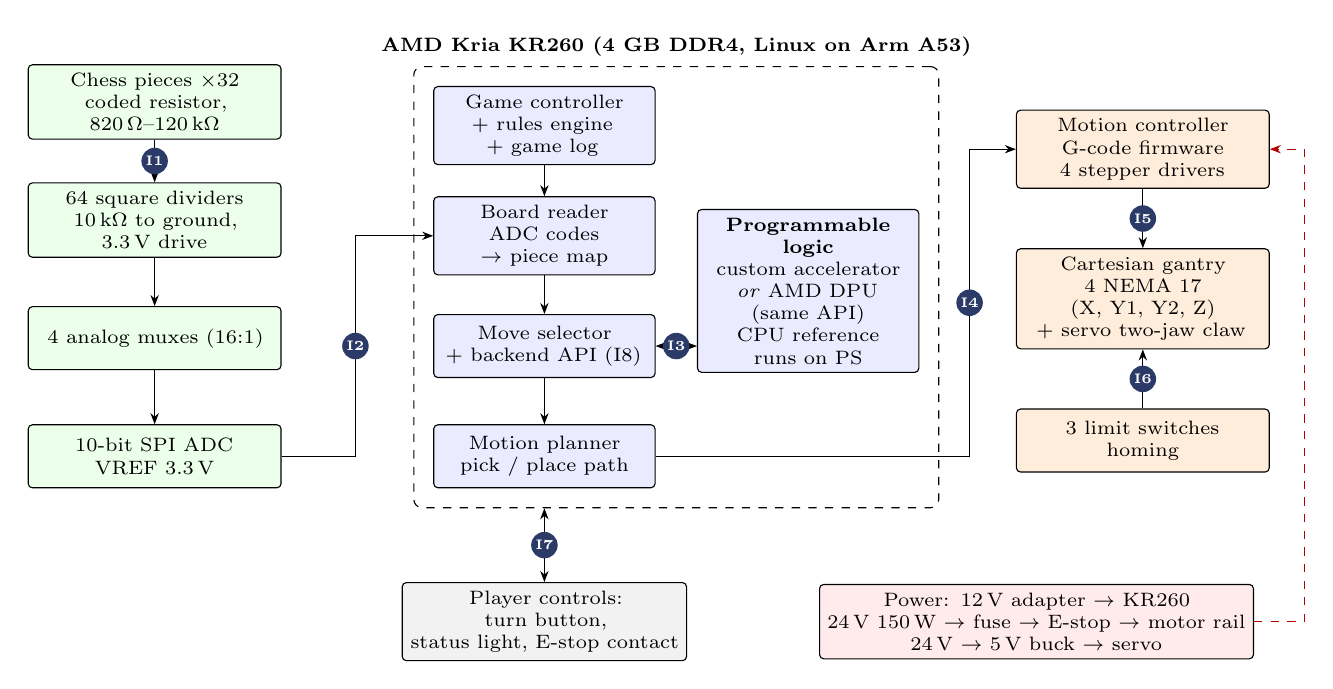
\begin{tikzpicture}[font=\scriptsize, >={Stealth[length=4pt]},
  box/.style={draw, rounded corners=1.5pt, align=center, inner sep=3pt, minimum height=0.8cm},
  sen/.style={box, fill=green!8, text width=3.0cm},
  ps/.style={box, fill=blue!8, text width=2.6cm},
  mot/.style={box, fill=orange!14, text width=3.0cm},
  badge/.style={circle, fill=navy, text=white, font=\tiny\bfseries, inner sep=0.8pt}]
  % sensing
  \node[sen] (pieces) at (0, 0) {Chess pieces $\times$32\\coded resistor, 820\,$\Omega$--120\,k$\Omega$};
  \node[sen] (div) at (0, -1.5) {64 square dividers\\10\,k$\Omega$ to ground, 3.3\,V drive};
  \node[sen] (mux) at (0, -3.0) {4 analog muxes (16:1)};
  \node[sen] (adc) at (0, -4.5) {10-bit SPI ADC\\VREF 3.3\,V};
  % processing system
  \node[ps] (ctl) at (4.95, -0.3) {Game controller\\+ rules engine + game log};
  \node[ps] (rd) at (4.95, -1.7) {Board reader\\ADC codes $\to$ piece map};
  \node[ps] (sel) at (4.95, -3.1) {Move selector\\+ backend API (I8)};
  \node[ps] (plan) at (4.95, -4.5) {Motion planner\\pick / place path};
  \node[ps, text width=2.6cm] (pl) at (8.3, -2.4) {\textbf{Programmable logic}\\custom accelerator\\\emph{or} AMD DPU\\(same API)\\CPU reference runs on PS};
  \node[draw, dashed, rounded corners=3pt, fit=(ctl)(plan)(pl), inner sep=7pt] (kria) {};
  \node[font=\scriptsize\bfseries, anchor=south] at (kria.north) {AMD Kria KR260 (4 GB DDR4, Linux on Arm A53)};
  % motion
  \node[mot] (mc) at (12.55, -0.6) {Motion controller\\G-code firmware\\4 stepper drivers};
  \node[mot] (gan) at (12.55, -2.5) {Cartesian gantry\\4 NEMA 17 (X, Y1, Y2, Z)\\+ servo two-jaw claw};
  \node[mot] (lim) at (12.55, -4.3) {3 limit switches\\homing};
  % bottom
  \node[box, fill=gray!10, text width=3.4cm] (ui) at (4.95, -6.6) {Player controls: turn button,\\status light, E-stop contact};
  \node[box, fill=red!8, text width=5.3cm] (pwr) at (11.2, -6.6) {Power: 12\,V adapter $\to$ KR260\\24\,V 150\,W $\to$ fuse $\to$ E-stop $\to$ motor rail\\24\,V $\to$ 5\,V buck $\to$ servo};
  % arrows
  \draw[->] (pieces) -- node[badge, pos=0.5] {I1} (div);
  \draw[->] (div) -- (mux);
  \draw[->] (mux) -- (adc);
  \draw[->] (adc.east) -- (2.55, -4.5) -- node[badge, pos=0.5] {I2} (2.55, -1.7) -- (rd.west);
  \draw[->] (ctl) -- (rd);
  \draw[->] (rd) -- (sel);
  \draw[->] (sel) -- (plan);
  \draw[<->] (sel.east) -- node[badge, pos=0.5] {I3} (sel.east -| pl.west);
  \draw[->] (plan.east) -- (10.35, -4.5) -- node[badge, pos=0.5] {I4} (10.35, -0.6) -- (mc.west);
  \draw[->] (mc) -- node[badge, pos=0.5] {I5} (gan);
  \draw[<-] (gan) -- node[badge, pos=0.5] {I6} (lim);
  \draw[<->] (ui) -- node[badge, pos=0.5] {I7} (kria.south -| ui);
  \draw[->, dashed, red!70!black] (pwr.east) -- (14.6, -6.6) -- (14.6, -0.6) -- (mc.east);
\end{tikzpicture}
\caption{System block diagram. Solid arrows are signals; the dashed arrow is motor power. Badges
match the interface IDs of the Technical Design Document: I1 piece-to-square contacts, I2 SPI to
ADC, I3 PS--PL link (AXI4-Lite, AXI DMA, interrupt), I4 USB serial G-code, I5/I6 drivers, servo and
switches, I7 player controls, I8 software backend API.}\label{fig:sys}
\end{figure}

\subsection{Key Design Decisions}

Table~\ref{tab:dec} summarizes the main choices and why we rejected the alternatives.

\begin{table}[H]
\centering\small
\caption{Design decisions and rejected alternatives.}\label{tab:dec}
\begin{tabularx}{\textwidth}{@{}P{2.7cm} P{3.0cm} L@{}}
\toprule
\textbf{Decision} & \textbf{Alternatives} & \textbf{Rationale} \\
\midrule
Resistor-coded pieces read by voltage dividers & Camera; RFID per square & A camera would compete with the benchmark for the KR260, and RFID needs an antenna per square. Resistors are passive and need one ADC. The 12 codes sit about 0.25 V apart and stay at least 0.18 V apart in the worst case (1\% resistors plus 100 $\Omega$ of contact and mux resistance), about 55 counts on the 10-bit ADC. \\
Cartesian gantry with claw & SCARA, CoreXY, delta; magnets under the board & Each axis has its own drive, so it is simple to build and debug. A claw lifts pieces over others. \\
G-code motion controller & Step pulses generated in the FPGA & Tested printer firmware handles step timing, and the PL stays free for the accelerator comparison. \\
Single inference per move, no search & Alpha-beta plus NNUE & A fixed workload we can benchmark, and human-like play at a chosen rating. \\
Legal-move masking & Trusting the network output & Every reply is legal even if the network is weak. \\
One software API (\texttt{load\_model}, \texttt{infer}, \texttt{stats}) & Separate code paths per backend & Only the backend changes between custom, DPU, and CPU, which keeps the comparison fair. \\
Time-multiplexed MAC array with on-chip memory & Fully unrolled dataflow & Fits the DSP and memory budget. The fallback is moving weights to block RAM or DDR. \\
\bottomrule
\end{tabularx}
\end{table}

\lead{Accelerator approach.} The PS loads the INT8 weights into on-chip UltraRAM once. One
matrix-multiply engine, a $64\times8$ array of DSP multiply-accumulate cells with one lane per
board square, is reused for every matrix multiply in the network. Separate units handle the
operations a plain MAC array cannot: requantization, softmax (through an exponential lookup table),
normalization, the activation function, and the geometric attention bias. Activations stay on chip
in small memory banks. The PS controls the accelerator through memory-mapped registers over
AXI4-Lite and exchanges data with it through an AXI DMA. For each move the PS sends the encoded
position, reads back the policy and win/draw/loss outputs, assembles one score for each of 4,352
encoded moves, masks the illegal ones, and picks. The DPU is INT8 only, has no native attention or
softmax, and streams weights from DDR. The benchmark will measure what those differences cost.

\subsection{Proof-of-Concept Demo (Status Meeting \#3 and Design Review, Dec.\ 4)}

The proof of concept shows that the four riskiest parts each work on their own before we integrate
them. We kept it narrow so we can finish it and show it live.

\begin{enumerate}[label=\textbf{PoC-\arabic*.}, leftmargin=3.6em]
\item \lead{Sensing.} The $2\times2$ test tile reads all 12 printed resistor-coded piece types and
  empty squares through the mux and ADC chain. We show the readings against the expected codes and
  a plot of reading margins.
\item \lead{Motion.} The printed servo claw grips, lifts, and releases each of the six piece shapes
  on a bench fixture, and we present the gantry design with its bill of materials. The gantry is
  not built yet, so powered pick-and-place and the emergency-stop test are January milestones.
\item \lead{Inference.} The Maia-style network runs on the KR260 through the DPU and on the CPU,
  and we report measured latency and the operations that fall back to the CPU. In simulation, the
  MAC array and matrix-multiply engine pass their self-checking testbenches, and we show their
  synthesis results.
\item \lead{Software.} The game controller plays a legal game in simulation by replaying PGN input,
  with the rules engine agreeing with python-chess.
\end{enumerate}

Stretch: one human move on the test tile, scanned and answered by the CPU backend.

\subsection{Minimum Viable Product (April 2027)}

The MVP is a complete, reproducible system. Everything below except the stretch goals is required.

\begin{itemize}
\item \lead{Game play.} Plays a full game against a human on a real board, handling captures,
  castling, en passant, and promotion, with checkmate and draw detection and a status light for
  every state (NFR-1, NFR-3, NFR-4).
\item \lead{Sensing.} 64-square scan with zero misreads over 1,000 scans. Unreadable squares are
  never reported as pieces (FR-SEN).
\item \lead{Verification and recovery.} Post-move rescan, one corrective move, then a request for
  human help (FR-VER).
\item \lead{Accelerator.} The custom accelerator chooses every robot move. It is bit-exact with the
  CPU integer reference on all golden vectors and meets timing, with no CPU computation between the
  input and output DMA transfers (FR-ACC, NFR-2).
\item \lead{Comparison.} One-command benchmark of the custom, DPU, and CPU backends with latency,
  energy per inference, utilization, and fallback operations (FR-BEN).
\item \lead{Safety.} Hardware emergency stop under 100 ms, and no pinch points reachable from the
  player's side (NFR-5).
\item \lead{Openness.} MIT-licensed repository and a published priced bill of materials (NFR-6,
  NFR-8).
\item \lead{Stretch goals.} Model-size sweep with an accuracy curve; swapping in Stockfish through
  the UCI interface (NFR-7); selectable ratings between 600 and 2600; underpromotion pieces.
\end{itemize}

\section{Risk Assessment}

Table~\ref{tab:risk} rates each risk for likelihood (L) and impact (I) as Low, Medium, or High,
with an early-warning trigger where one is useful. The first three drive the schedule.

\begin{table}[H]
\centering\small
\caption{Risk register.}\label{tab:risk}
\begin{tabularx}{\textwidth}{@{}l P{3.9cm} c c L@{}}
\toprule
\textbf{ID} & \textbf{Risk} & \textbf{L} & \textbf{I} & \textbf{Mitigation and contingency} \\
\midrule
R1 & Network spec slips, or the final model outgrows on-chip memory (weights already use 49 of 64 UltraRAM) & H & H & Every size in the RTL is a parameter; written spec with golden vectors; move the attention-bias templates to block RAM, then tile from DDR. Trigger: no frozen spec by the end of December. \\
R2 & Accelerator misses timing, exceeds fabric resources, or is not bit-exact & M & H & Synthesis results logged for every block as it is written; layer-by-layer golden checks in simulation; the DPU and CPU backends keep the product playable. \\
R3 & Poor contact gives a wrong piece code & M & H & Test tile before building 64 squares; double scan before accepting; readings more than 0.09 V from every code flagged unreadable; redesign the contact pads if margins are thin. \\
R4 & Piece slips in the claw or pickup is unreliable & M & M & Claw seats under a cone on every piece instead of squeezing; rescan and one retry; adjustable jaw geometry. \\
R5 & Placement error from belt backlash, frame flex, or calibration drift & M & M & Two-corner calibration saved across power cycles; stiff frame; rehoming each game; measure over 100 placements. \\
R6 & The gantry is not built and its parts are not ordered & H & M & Ask the campus makerspaces for a used 3D printer for parts in December; order the rest before winter break; game software develops against PGN replay in the meantime. \\
R7 & DPU cannot run attention operations, making the baseline look unfair & M & M & Report CPU fallbacks and transfer costs, and state the comparison conditions. The fallback list is a result we want to report anyway. \\
R8 & Toolchain or model licensing, or tool versions, block the flow & L & H & Confirm Vivado, Vitis AI, and Maia-3 licensing now; pin tool versions; build from scripts. \\
R9 & Injury or damage from a moving gantry, especially around children & L & H & Hardware e-stop independent of software; no motion during the player's turn; controls outside the gantry frame; guarded pinch points; 24 V only. \\
R10 & Part lead times, budget overruns, or lost lab time & M & M & Order long-lead parts early; spares in the budget; prototype with 3D-printed parts; keep sponsors informed. \\
R11 & Teammate unavailability or ownership gaps & M & M & Named owners per workstream, one shared repository, and written interface specs so a teammate can pick up a task. \\
R12 & Small model plays poorly & M & L & Legal-move masking guarantees legality; the comparison stays valid; a sweep documents the accuracy tradeoff. \\
\bottomrule
\end{tabularx}
\end{table}

\section{Ethics and Social Impact}

\lead{Physical safety.} A moving gantry with a closing claw is a hazard, particularly at an expo.
We apply the stop-function principles of ISO 13850~\cite{iso13850}: a latching, normally-closed
emergency stop removes motor power in hardware within 100 ms, independent of the KR260, while the
computer stays powered so the game state is preserved. The robot never moves during the player's
turn, the player's controls sit outside the gantry frame, and the motor rail is low voltage (24 V)
and fused. Safety is a tested requirement (NFR-5).

\lead{Dual use of human-like engines.} A model that imitates human play could be misused to cheat
online or over the board. Our system is a self-contained physical board with no channel to an
opponent, and we do not distribute tools for transmitting moves. The repository will state the
intended use.

\lead{Openness, access, and licensing.} Releasing everything under the MIT license with a priced
bill of materials makes the project easier for students and hobbyists to build. It also means we
have to check that the Maia weights and training data~\cite{maia, maia3} allow redistribution,
credit them, and keep vendor IP out of the repository. The DPU and Vitis AI are used under AMD's
terms and are not redistributed.

\lead{Research integrity.} FR-BEN-5 requires us to write the benchmark report even if it favors the
vendor DPU or the CPU, in line with the IEEE Code of Ethics~\cite{ieee}. We state the measurement
conditions (instrument, sample rate, idle power subtraction) so the results can be reproduced, and
we will not pick favorable positions or runs.

\lead{Privacy and data.} The robot stores only game logs and timing on a local microSD card. It has
no camera or microphone and needs no network, so it collects no personal data. If we later gather
feedback from expo players, we will first confirm whether human-subject review applies.

\lead{Fairness and user experience.} Rating-matched play can make the game more welcoming to
beginners. A human-like model also reflects its training data, which may skew toward online play at
particular rating bands, so we will report which ratings we validated.

\lead{Environmental impact.} 3D printing and electronics create plastic and electronic waste. We
use passive components for sensing, reuse prototypes, and document the design so the hardware can
be repaired.

\section{Testing Plan}

\subsection{Test Types and Methods}

Every requirement in the Design Requirements Document names a verification method (Test,
Demonstration, Inspection, or Analysis), and we keep a requirements-to-test traceability matrix.
Testing goes from isolated parts to the full system.

\begin{itemize}
\item \lead{Unit tests (software).} Rules engine, board reader, move encoder, and move selector
  against python-chess on at least 10,000 positions (FR-GAM-2, FR-ENG-1/2), and PGN replay over at
  least 1,000 recorded games in simulation mode (FR-GAM-6).
\item \lead{Hardware simulation.} Every RTL module has a self-checking testbench, run in Icarus
  Verilog or the Vivado simulator. Each unit is checked against a bit-accurate Python integer model
  on golden vectors, layer by layer, and a mismatch reports the first failing layer (FR-ACC-3).
\item \lead{Hardware-in-the-loop.} The same golden vectors run on the KR260 through the custom
  accelerator, DPU, and CPU backends. The custom accelerator must match the integer reference bit
  for bit. The DPU and floating-point CPU paths, whose number formats differ, must choose the same
  highest-scoring legal move.
\item \lead{Integration tests.} Sensing to controller (scan, decode the move, reject illegal
  moves), controller to motion (G-code sequences for each move type), and the verify-and-retry loop
  with injected faults such as a displaced piece or an unreadable square (FR-VER, FR-ENG-4).
\item \lead{Performance testing.} The benchmark harness times at least 1,000 inferences per backend
  and reports latency, throughput, and energy per inference, computed as (active power minus idle
  power) $\times$ latency. The instrument and sample rate are recorded (FR-BEN-3/4).
\item \lead{Physical and mechanical tests.} Scans with each piece type on every square (1,000
  scans, 10 or more positions); repeated pick-and-place over 100 placements within 5 mm; 50
  consecutive moves in 3 of 3 trials.
\item \lead{Safety tests.} Emergency stop pressed mid-move, with the motor-rail cutoff time
  measured on an oscilloscope (NFR-5), and confirmation that no axis moves during the human's turn.
\item \lead{Acceptance test.} A scripted full game covering every move type, then an unscripted
  game against a human volunteer.
\end{itemize}

\subsection{Process and Tooling}

\begin{itemize}
\item \lead{Source control.} All RTL, software, CAD, and scripts live in one Git repository, with a
  folder and an owner per subsystem. A change to a shared file (the parameter package, the numerics
  spec, the register map) needs its owner's approval.
\item \lead{Automated testing and CI.} Testbenches and the CAD fit checks run from scripts today.
  In January we plan to add a GitHub Actions pipeline that runs linting, the python-chess
  cross-checks, PGN replay, and the RTL simulation regression on every pull request.
\item \lead{Reproducible builds.} Vivado is pinned at 2023.2 and the project is generated from a
  Tcl script and never committed. Bitstreams, weights, and golden vectors will be versioned
  together so a result can be reproduced. Synthesis results for each block are logged in the
  repository with the commit they came from.
\item \lead{Golden vectors.} For each unit we write the Python integer reference before the RTL.
  The same file generates the test vectors and the expected outputs, and simulation, the board, and
  the CPU reference all check against it.
\item \lead{Logging and data.} Every move records the backend and inference latency, and benchmark
  results are saved as files and committed.
\end{itemize}

\subsection{Sections Not Applicable or Changed}

No milestones have been removed from the course schedule for our team. The project needs no
regulatory approvals and involves no human-subject research or customer data at this stage. The
budget is preliminary until we have vendor prices.

\begin{thebibliography}{99}
\small
\setlength{\itemsep}{0.15em}

\bibitem{kr260} AMD, ``Kria KR260 Robotics Starter Kit User Guide,'' UG1092. [Online]. Available:
\url{https://docs.amd.com/r/en-US/ug1092-kr260-starter-kit}. [Accessed: Oct. 26, 2026].

\bibitem{maia} R. McIlroy-Young, S. Sen, J. Kleinberg, and A. Anderson, ``Aligning superhuman AI
with human behavior: Chess as a model system,'' in \emph{Proc. 26th ACM SIGKDD Int. Conf. Knowl.
Discovery Data Mining}, 2020, pp. 1677--1687.

\bibitem{chessformer} D. Monroe, G. Eilender, P. Chalmers, Z. Tang, and A. Anderson, ``Chessformer:
A unified architecture for chess modeling,'' arXiv:2605.19091, May 2026.

\bibitem{dpu} AMD, ``DPUCZDX8G for Zynq UltraScale+ MPSoCs Product Guide,'' PG338. [Online].
Available: \url{https://docs.amd.com/r/en-US/pg338-dpu}. [Accessed: Oct. 26, 2026].

\bibitem{maia3} CSSLab, ``maia3,'' GitHub repository. [Online]. Available:
\url{https://github.com/CSSLab/maia3}. [Accessed: Oct. 26, 2026].

\bibitem{marlin} Marlin Firmware, ``G-code reference.'' [Online]. Available:
\url{https://marlinfw.org/docs/gcode/}. [Accessed: Nov. 8, 2026].

\bibitem{squareoff} Square Off, ``Square Off self-moving chess boards.'' [Online]. Available:
\url{https://squareoffnow.com}. [Accessed: Nov. 18, 2026].

\bibitem{dgt} Digital Game Technology, ``DGT electronic chess boards.'' [Online]. Available:
\url{https://digitalgametechnology.com}. [Accessed: Nov. 27, 2026].

\bibitem{chessnut} Chessnut, ``Chessnut electronic chess boards.'' [Online]. Available:
\url{https://www.chessnutech.com}. [Accessed: Nov. 27, 2026].

\bibitem{stockfish} The Stockfish developers, ``Stockfish.'' [Online]. Available:
\url{https://stockfishchess.org}. [Accessed: Nov. 27, 2026].

\bibitem{alphazero} D. Silver \emph{et al.}, ``A general reinforcement learning algorithm that
masters chess, shogi, and Go through self-play,'' \emph{Science}, vol. 362, no. 6419,
pp. 1140--1144, 2018.

\bibitem{deepblue} M. Campbell, A. J. Hoane Jr., and F.-h. Hsu, ``Deep Blue,'' \emph{Artif.
Intell.}, vol. 134, nos. 1--2, pp. 57--83, 2002.

\bibitem{finn} Y. Umuroglu \emph{et al.}, ``FINN: A framework for fast, scalable binarized neural
network inference,'' in \emph{Proc. ACM/SIGDA Int. Symp. Field-Programmable Gate Arrays (FPGA)},
2017, pp. 65--74.

\bibitem{hls4ml} J. Duarte \emph{et al.}, ``Fast inference of deep neural networks in FPGAs for
particle physics,'' \emph{J. Instrum.}, vol. 13, no. 7, Art. no. P07027, 2018.

\bibitem{jacob} B. Jacob \emph{et al.}, ``Quantization and training of neural networks for
efficient integer-arithmetic-only inference,'' in \emph{Proc. IEEE/CVF Conf. Comput. Vis. Pattern
Recognit. (CVPR)}, 2018, pp. 2704--2713.

\bibitem{horowitz} M. Horowitz, ``Computing's energy problem (and what we can do about it),'' in
\emph{IEEE Int. Solid-State Circuits Conf. (ISSCC) Dig. Tech. Papers}, 2014, pp. 10--14.

\bibitem{iso13850} \emph{Safety of Machinery---Emergency Stop Function---Principles for Design},
ISO 13850, 2015.

\bibitem{ieee} IEEE, ``IEEE Code of Ethics.'' [Online]. Available:
\url{https://www.ieee.org/about/corporate/governance/p7-8.html}. [Accessed: Nov. 18, 2026].

\end{thebibliography}

\end{document}
